\documentclass{article}
\usepackage{tikz}

\begin{document}

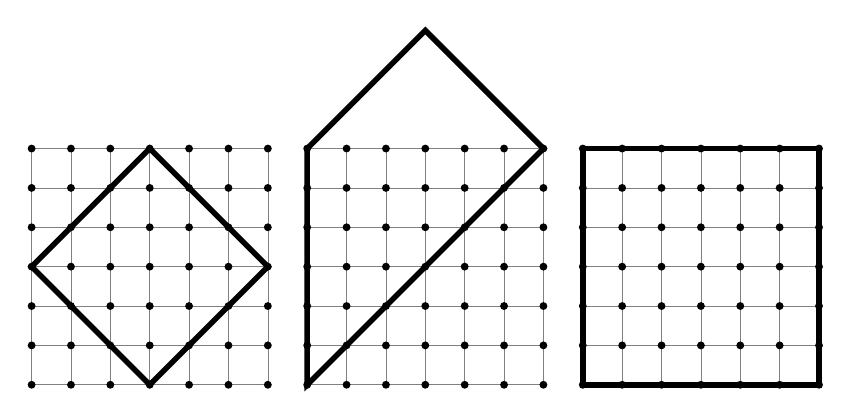
\begin{tikzpicture}[scale=0.5]
    % Grid 1
    \draw[help lines] (0,0) grid (6,6);
    \foreach \x in {0,...,6} {
        \foreach \y in {0,...,6} {
            \fill (\x,\y) circle (0.1);
        }
    }
    \draw[line width=2pt] (0,3) -- (3,6) -- (6,3) -- (3,0) -- cycle;

    % Grid 2
    \draw[help lines] (7,0) grid (13,6);
    \foreach \x in {7,...,13} {
        \foreach \y in {0,...,6} {
            \fill (\x,\y) circle (0.1);
        }
    }
    \draw[line width=2pt] (7,0) -- (10,3) -- (13,6) -- (10,9) -- (7,6) -- cycle;

    % Grid 3
    \draw[help lines] (14,0) grid (20,6);
    \foreach \x in {14,...,20} {
        \foreach \y in {0,...,6} {
            \fill (\x,\y) circle (0.1);
        }
    }
    \draw[line width=2pt] (14,0) -- (14,6) -- (20,6) -- (20,0) -- cycle;
\end{tikzpicture}

\end{document}